\documentclass[a4paper,10pt, DIV14]{scrartcl}

\usepackage[utf8x]{inputenc}
\usepackage{graphicx}
\usepackage{wrapfig}


\pdfinfo{%
  /Title    (Remapping Algorithm in prepicon)
  /Author   (Florian Prill)
}
\pagestyle{empty}

\begin{document}

\subsection*{Technical Notes: Conservative Remapping Algorithm in ICON}

\emph{--- Initial revision of this document: 2012-11-13, F.\ Prill, DWD ---}\\

As part of the \texttt{prep\_icon} binary, a 1$^{st}$ order area-weighted remapping
is available in the ICON code.
The algorithm shares the basic mesh data structure and a number of subroutines with the 
model sources.
A similar non-distributed algorithm is part of the climate data operators (CDOs).


\subsubsection*{General algorithm}

\begin{wrapfigure}{r}{0.37\textwidth}
%\begin{figure}[b!]
 \begin{center}
  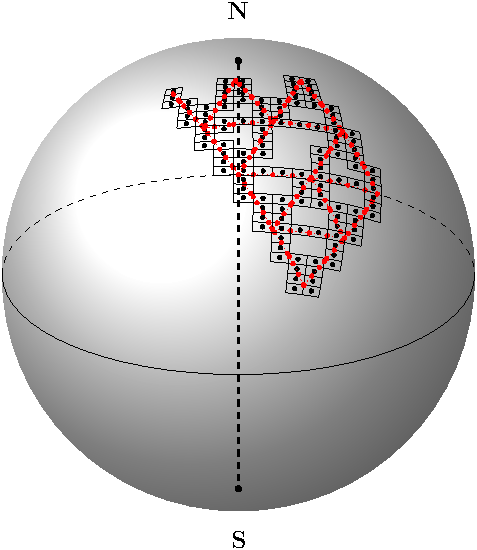
\includegraphics[width=0.33\textwidth]{remap_intersect.pdf}
 \end{center}
 \setcaphanging
 \setcapindent*{2em}
 \caption{Clipping algorithm, triangulation intersecting a regular grid.}
 \label{fig:intersection}
%\end{figure}
\end{wrapfigure}

The implementation can be applied to general unstructured grids. 
The algorithm itself has been described in detail in \cite{Jones1999}.
It yields conservative interpolation stencils of non-constant size.

Instead of computing the area integrals of overlap regions between the cells of the
source and destination grid, the method reduces this task to line
intersection and integration by applying the divergence theorem in spherical coordinates.
The algorithm operates on latitude-longitude coordinates and uses a
Lambert equivalent azimuthal projection in the pole regions.
See Fig.~\ref{fig:intersection} for an illustration of the clipping algorithm.

For the sake of simplicity, weights for both remapping directions are
computed during the setup phase.
The special case of surface pressure fields contains an (experimental) hydrostatic correction.


\subsubsection*{Current state}

The implementation is in a first release state.
Without any specific technical reason it is currently restricted to first-order accuracy.
The code is primarily aimed at IFS input data and can handle global regular grids in
GRIB2 and NetCDF file format, and local or global ICON triangular grids in NetCDF format.
File I/O is fully synchronous and writes NetCDF format (using the CDI).


\subsubsection*{Differences to the CDO remapping algorithm}

The remapping scheme has been implemented entirely in Fortran~90/95.
The method allows for a hybrid MPI/OpenMP parallelization.
The weight computation and the interpolation do not require global fields
and should therefore have no practical limit on the number of MPI tasks.
Some short-cuts like generalized near-neighbor access trees (GNATs) and
lookup tables are used to increase performance of the weight computation.
The method exploits the structure in regular grids.
For efficiency reasons, the stencil is decomposed into a static, fixed-size
table and a sequential list containing those weights that do not fit into
the simple stencil size.


\subsubsection*{Parallelization}

Grid cells are distributed over all processes according to their \emph{latitude}.
No global three dimensional fields are stored or exchanged.
The decomposition of the destination grid also implies a partitioning of the
source grid:
Each MPI task stores only a covering subset  of the source grid.

The multi-threaded weight computation stores results in \emph{binomial heaps}, i.e.\ tree-like
data structures with a special ordering.
An efficient merging algorithm finally collects these binomial heaps on the master thread.


\bibliographystyle{alpha} 
\begin{thebibliography}{1}
  \bibitem[Jones1999]{Jones1999} Jones, P. W.: 
                      \emph{First- and Second-Order Conservative Remapping Schemes for Grids in Spherical Coordinates.}
                      Mon. Wea. Rev., 1999, 127, 2204-2210
\end{thebibliography}

\end{document}
